\documentclass[12pt]{article}
\usepackage{setspace}
\usepackage{graphicx}
\setstretch {1.25} 
\usepackage{geometry}
\geometry{papersize={21cm,29.7cm}}
\geometry{left=2.5cm,right=2.5cm,top=3cm,bottom=3cm}
\usepackage{fancyhdr}
\usepackage{listings}
\usepackage{color}
\definecolor{black}{rgb}{0,0,0}
\definecolor{olivegreen}{RGB}{112,161,71}
\definecolor{lakeblue}{RGB}{0,127,255}
\definecolor{orange}{RGB}{255,139,0}
\definecolor{purple}{RGB}{102,0,255}
\pagestyle{fancy}
\lhead{\author}
\chead{\date}
\lfoot{}
\cfoot{\thepage}
\rfoot{}
\renewcommand{\headrulewidth}{0.4pt}
\renewcommand{\headwidth}{\textwidth}
\renewcommand{\footrulewidth}{0pt}
\usepackage{xeCJK}
\setCJKmainfont{SimSun}
\XeTeXlinebreaklocale “zh”
\XeTeXlinebreakskip = 0pt plus 1pt
\title{OpenGL作业报告\  C类第2题}
\author{夏斐 2012011417}

\date{\today}
\begin{document}
\maketitle
\linespread {1}
\section{实验环境}
本作业在Mac OS X10.8.2系统下用Xcode完成,程序框架是命令行,用到了系统原生支持的OpenGL和GLUT框架,如图所示:
\begin{center}
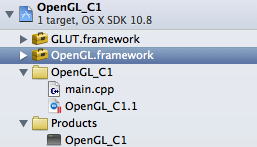
\includegraphics[width = 2.5in]{environment.png} 
\end{center}
\par
\section{实验原理}
上一次作业我们绘制了基本的平面图形,这一次作业在上一次的基础上扩展即可,首先,我们绘制三维物体的多个面,这样就相当于完成了三维图形的绘制。旋转等操作利用变换矩阵,和第一次比较类似。
\par但是我们需要注意有一些不同的地方,首先,为了使三维图形看上去更立体,我们需要设置设置透视投影矩阵,这个函数在reshape时调用,这样我们在改变窗体大小时也不会变形。其次,为了保证在不同面上我们看到某个点的颜色是一样的,在绘制面时我们需要使每个点颜色相同。
\section{实验步骤}
主函数如下,注意到和上一次相比,我们额外增加了glutReshaoefunction,并且在其中设置透视投影矩阵。
\begin{lstlisting}[
language=C++, 
breakatwhitespace=false,
label=lst:helloworld, 
caption=Main, 
showspaces=false,
showlines = false,
showstringspaces  = false,
%basicstyle=\ttfamily,
identifierstyle = \color{purple},
stringstyle = \ttfamily,
keywordstyle=\color{lakeblue}\bfseries,
numberstyle = \color{purple}\bfseries,
commentstyle=\color{olivegreen}]
int main(int argc, char ** argv)
{
    glutInit(&argc, argv);
    glutInitDisplayMode(GLUT_DOUBLE|GLUT_RGBA|GLUT_DEPTH);
    glutInitWindowSize(400 , 400);
    glutInitWindowPosition(100, 100);
    glutCreateWindow("xf");
    glutSetCursor(GLUT_CURSOR_CROSSHAIR);
    glDepthFunc(GL_LEQUAL);
    glutKeyboardFunc(&processNormalKeys);
    glutDisplayFunc(&myDisplay);
    glutIdleFunc(&myDisplay);
    glutReshapeFunc(&reshape);
    glutMainLoop();
    return 0;
}\end{lstlisting}
\par
显示函数如下,其中绘制对象部分比较冗长,已经省略。
\begin{lstlisting}[
language=C++, 
breakatwhitespace=false,
label=lst:helloworld, 
caption=Display, 
showspaces=false,
showlines = false,
showstringspaces  = false,
%basicstyle=\ttfamily,
identifierstyle = \color{purple},
stringstyle = \ttfamily,
keywordstyle=\color{lakeblue}\bfseries,
numberstyle = \color{purple}\bfseries,
commentstyle=\color{olivegreen}]
void myDisplay()
{
    if (paint) glShadeModel(GL_SMOOTH);
         else glShadeModel(GL_FLAT);
    glEnable(GL_DEPTH_TEST);
    glClear(GL_COLOR_BUFFER_BIT|GL_DEPTH_BUFFER_BIT);
    glLoadIdentity();
    //glScalef(0.2, 0.2, 0.2);
    glTranslatef(1,2,3);
    glTranslatef(0, 0, -10.0f);
    glRotatef(angle, 1, 0, 0.0);
   //Draw The object
    glutSwapBuffers();
    angle-=0.05;
}
\end{lstlisting}
期中各参数的取值符合题目中的要求,我们在旋转之前,先移动到了坐标$(1,2,3)$的位置,为了使物体看上去不太大,我们又向屏幕中移动了10个单位。旋转的部分我们用了glRotate,其中第一个参数为1说明是围绕x轴旋转。
\par
锥体的显示与立方体的显示类似,不同的地方是围绕y轴旋转,我们只需要将glRotate的第二个参数改为1,第一个参数改为0即可。\par
我们用一个键盘事件来切换两种着色模式:
\begin{lstlisting}[
language=C++, 
breakatwhitespace=false,
label=lst:helloworld, 
caption=Keyevent, 
showspaces=false,
showlines = false,
showstringspaces  = false,
%basicstyle=\ttfamily,
identifierstyle = \color{purple},
stringstyle = \ttfamily,
keywordstyle=\color{lakeblue}\bfseries,
numberstyle = \color{purple}\bfseries,
commentstyle=\color{olivegreen}]
void processNormalKeys(unsigned char key, int x, int y) {
    
    if (key == ' ')
        paint  = !paint;
}\end{lstlisting}
\section{效果展示}
立方体平滑着色效果图:
\begin{center}
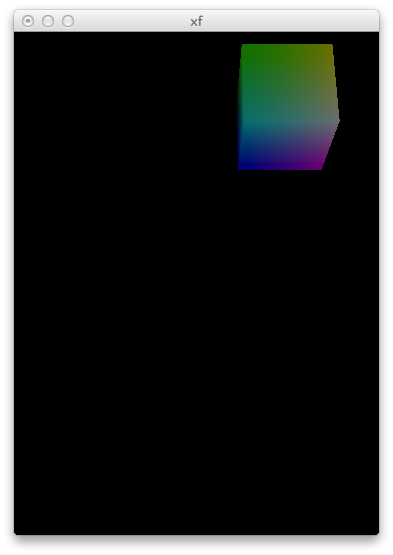
\includegraphics[width = 2.5in]{1.png} 
\end{center}
立方体单色着色效果图
\begin{center}
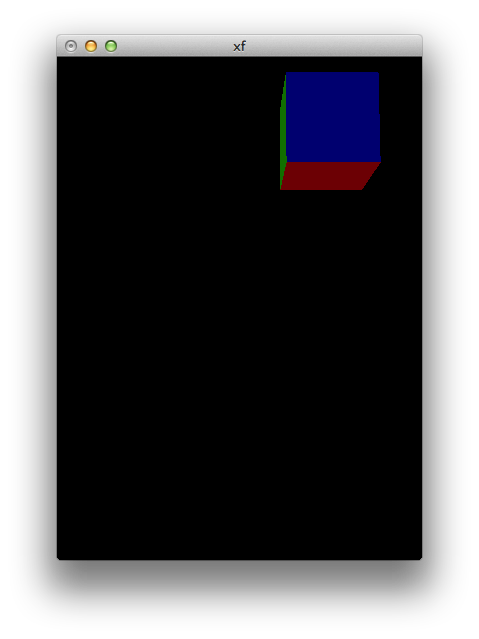
\includegraphics[width = 2.5in]{2.png} 
\end{center}
锥体平滑着色效果图
\begin{center}
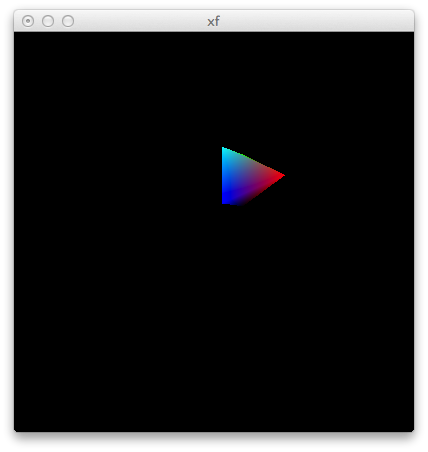
\includegraphics[width = 2.5in]{3.png} 
\end{center}
锥体单色效果图
\begin{center}
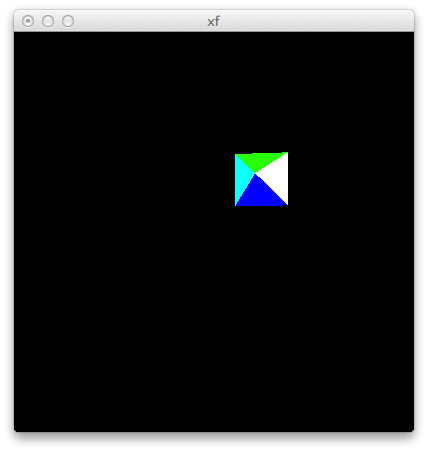
\includegraphics[width = 2.5in]{4.png} 
\end{center}
\section{参考文献}
[1]来自百度文库 OpenGL入门教程(精)

[2]Nehe OpenGL中文教程
\section{个人信息}
 \noindent
夏斐\\
清华大学 自动化系 2012级\\
手机:(+86)15652799536\\
邮箱:xf1280@gmail.com\\
\end{document}